%\documentclass{cumcmthesis}
\documentclass[withoutpreface,bwprint]{cumcmthesis} %去掉封面与编号页,电子版提交的时候使用。
\usepackage[final]{pdfpages}
\usepackage[linesnumbered,boxed,ruled,commentsnumbered]{algorithm2e}
\usepackage[framemethod=TikZ]{mdframed}
\usepackage{url}   % 网页链接
\usepackage{subcaption} % 子标题
\title{}
\tihao{A}
\baominghao{}
\schoolname{杭州电子科技大学}
\membera{ }
\memberb{ }
\memberc{ }
\supervisor{ }
\yearinput{2020}
\monthinput{08}
\dayinput{22}
\renewcommand\thesection{\arabic{section}.}

\begin{document}


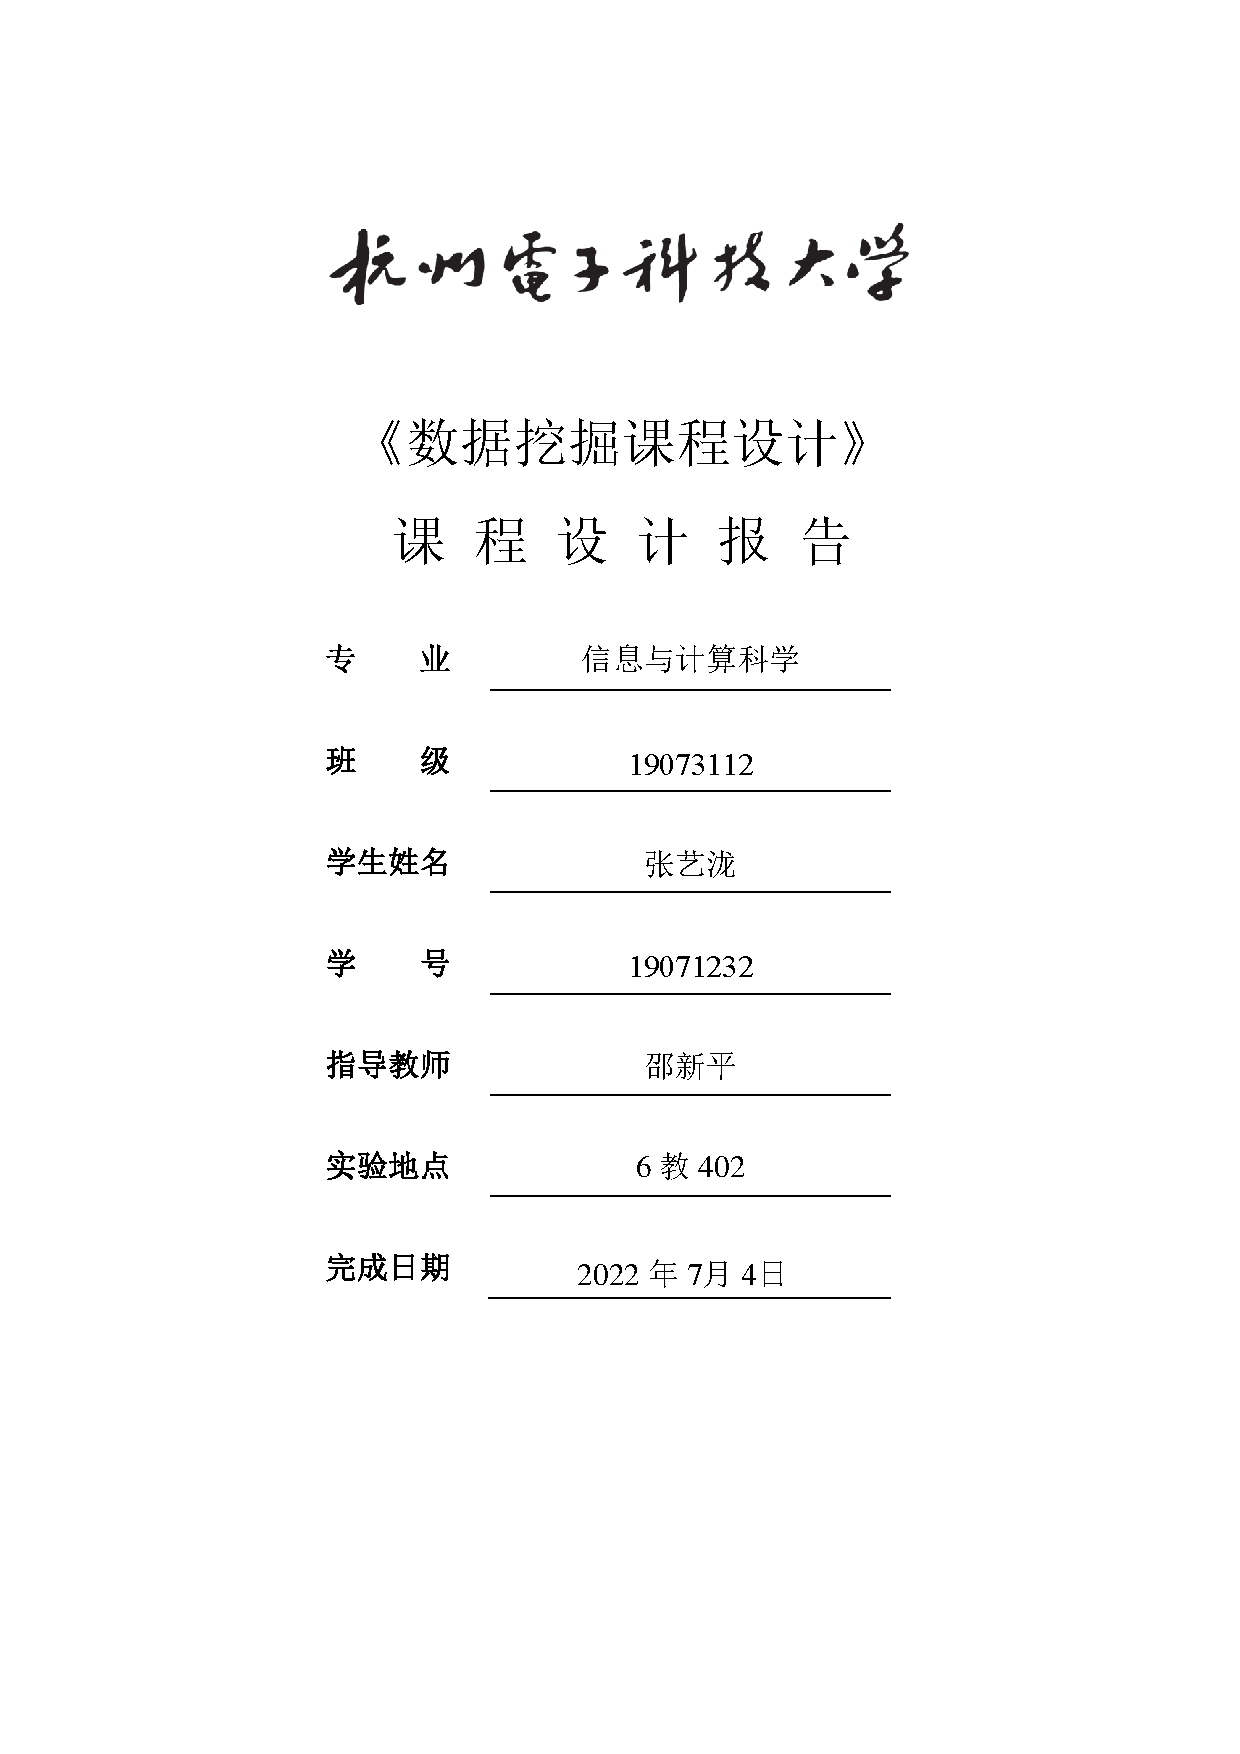
\includepdf{封面.pdf} 
\newpage

%目录
\tableofcontents

\newpage
\section{水质图片分类}
\subsection{数据集介绍}
\par 该数据集为某湖水样本,共203张图片,由类别+下划线+序号命名。
\begin{figure}[H]
	\centering
	\begin{minipage}[t]{0.48\textwidth}
		\centering
		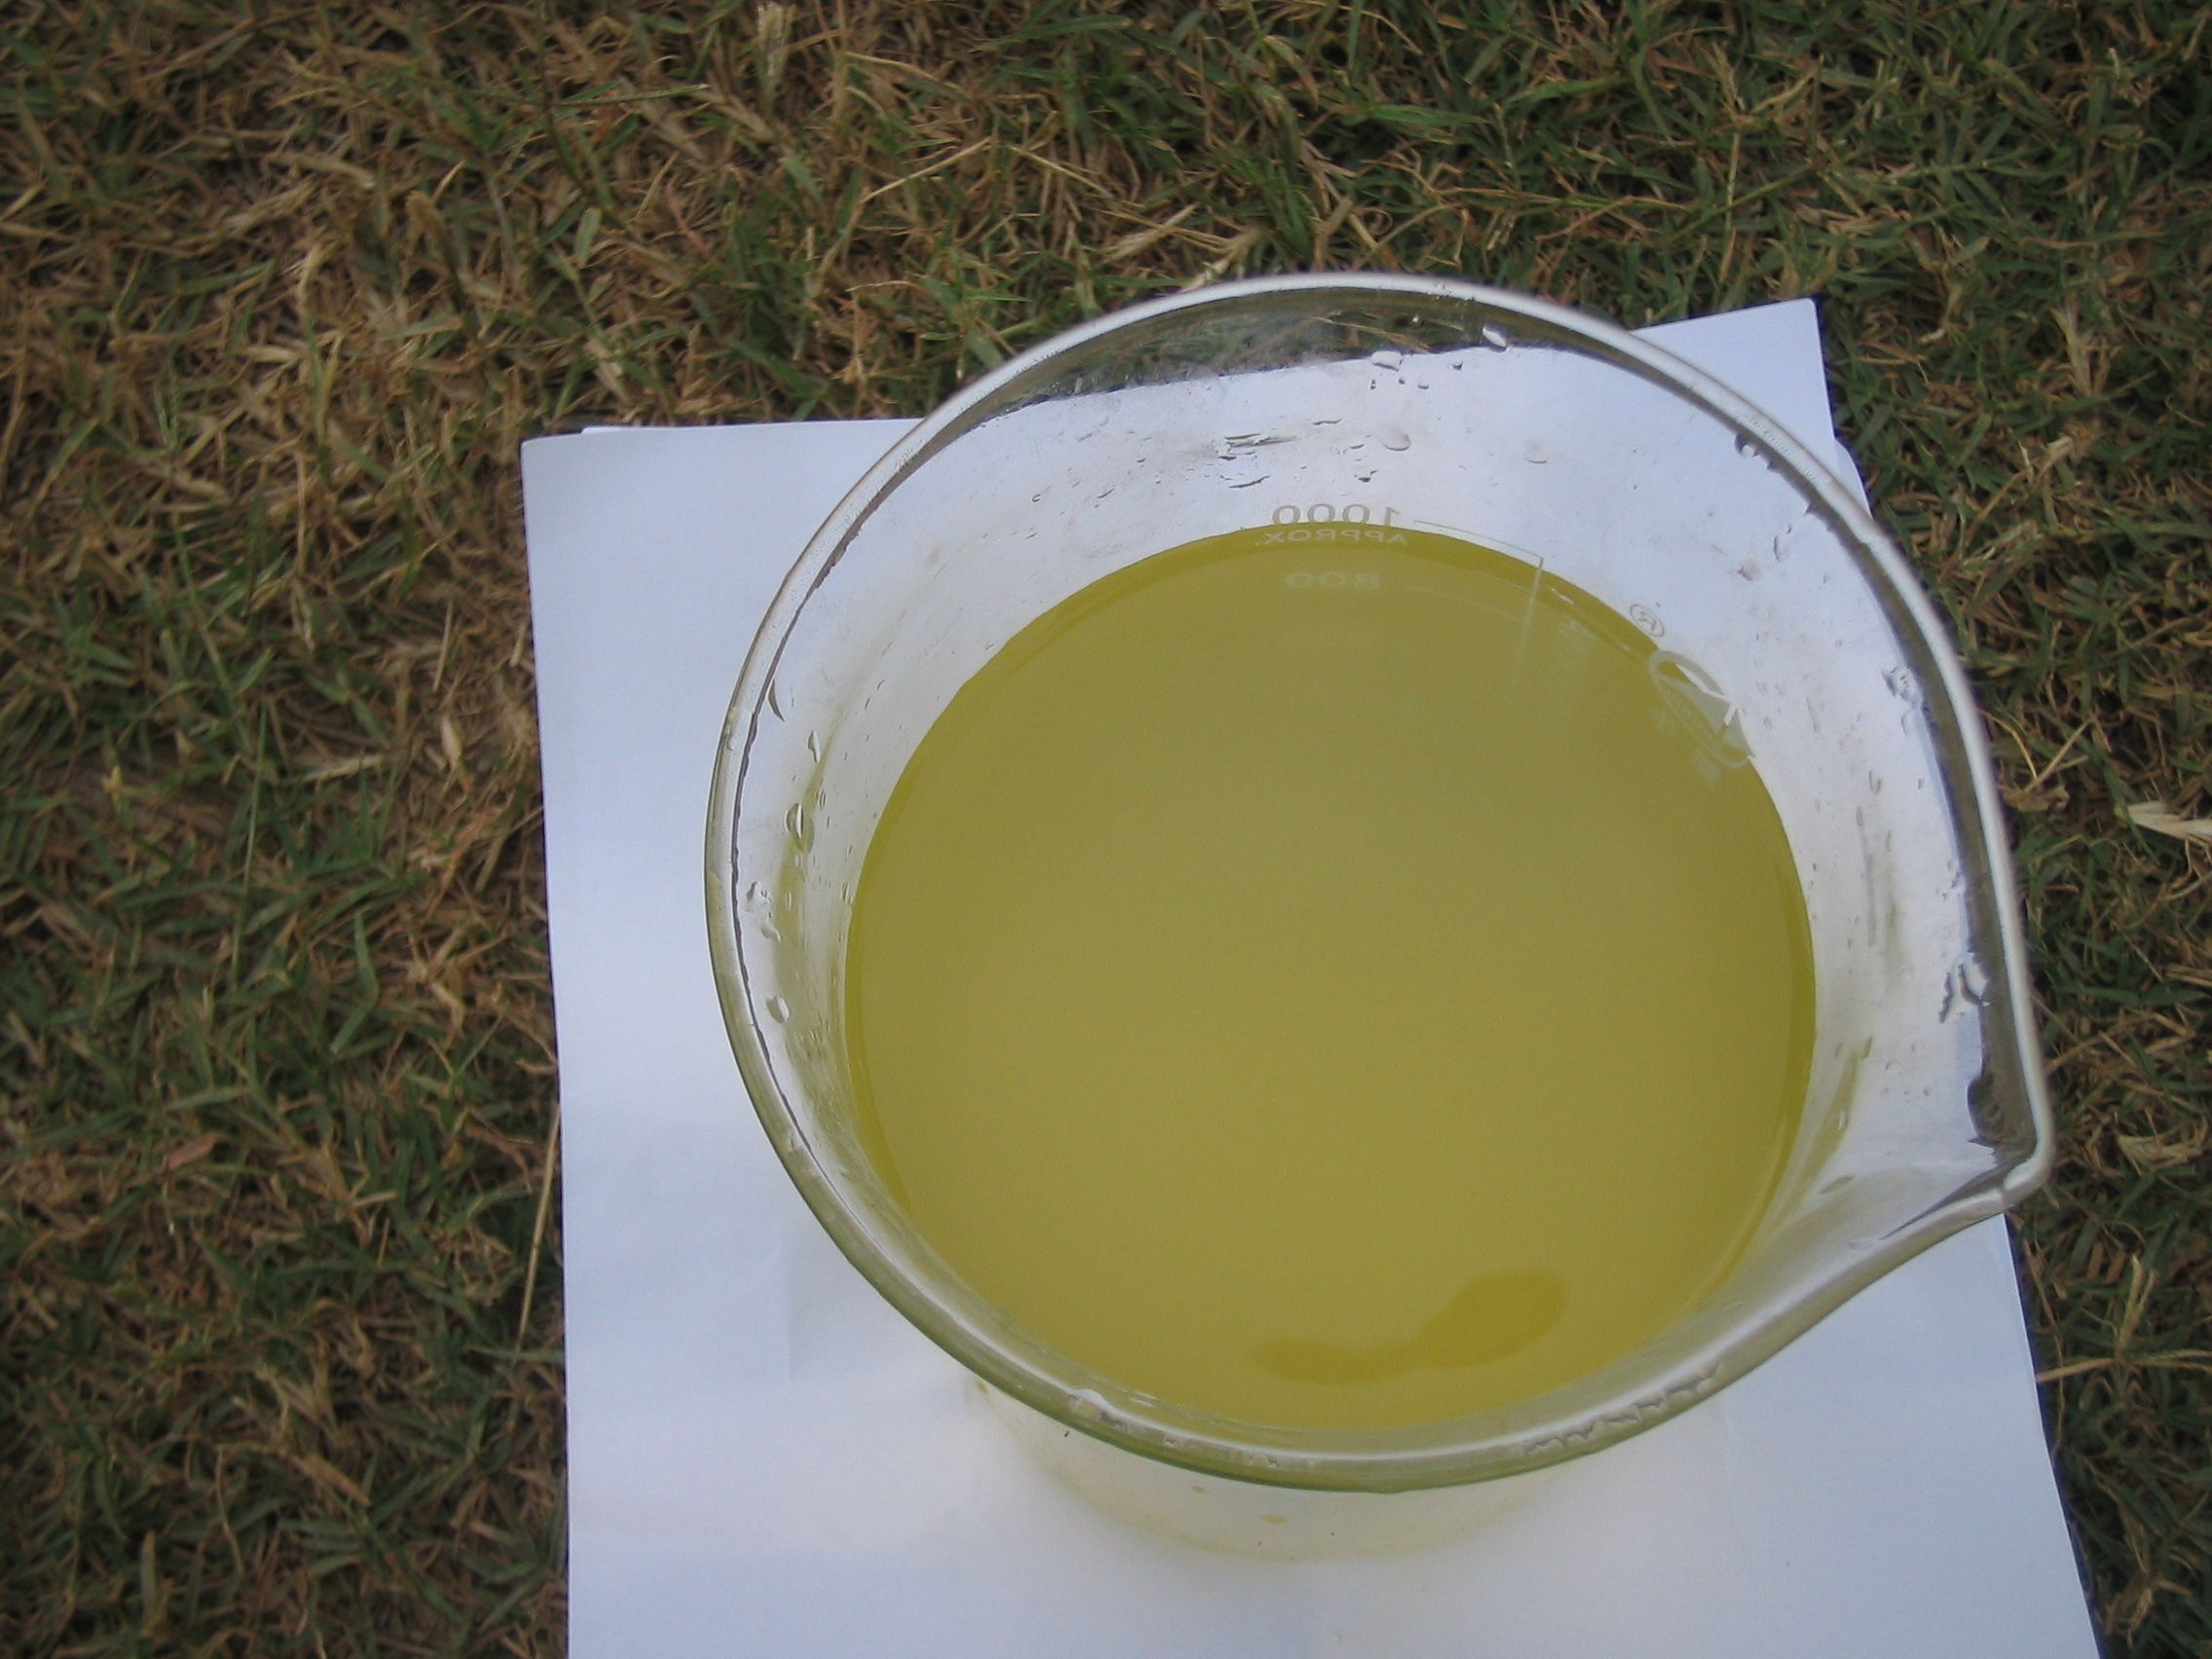
\includegraphics[width=6.3cm]{1_2.jpg}
		\centerline{$\ \ \ \ \ \ \ \ \ \ $(a)}
	\end{minipage}
	\begin{minipage}[t]{0.48\textwidth}
		\centering
		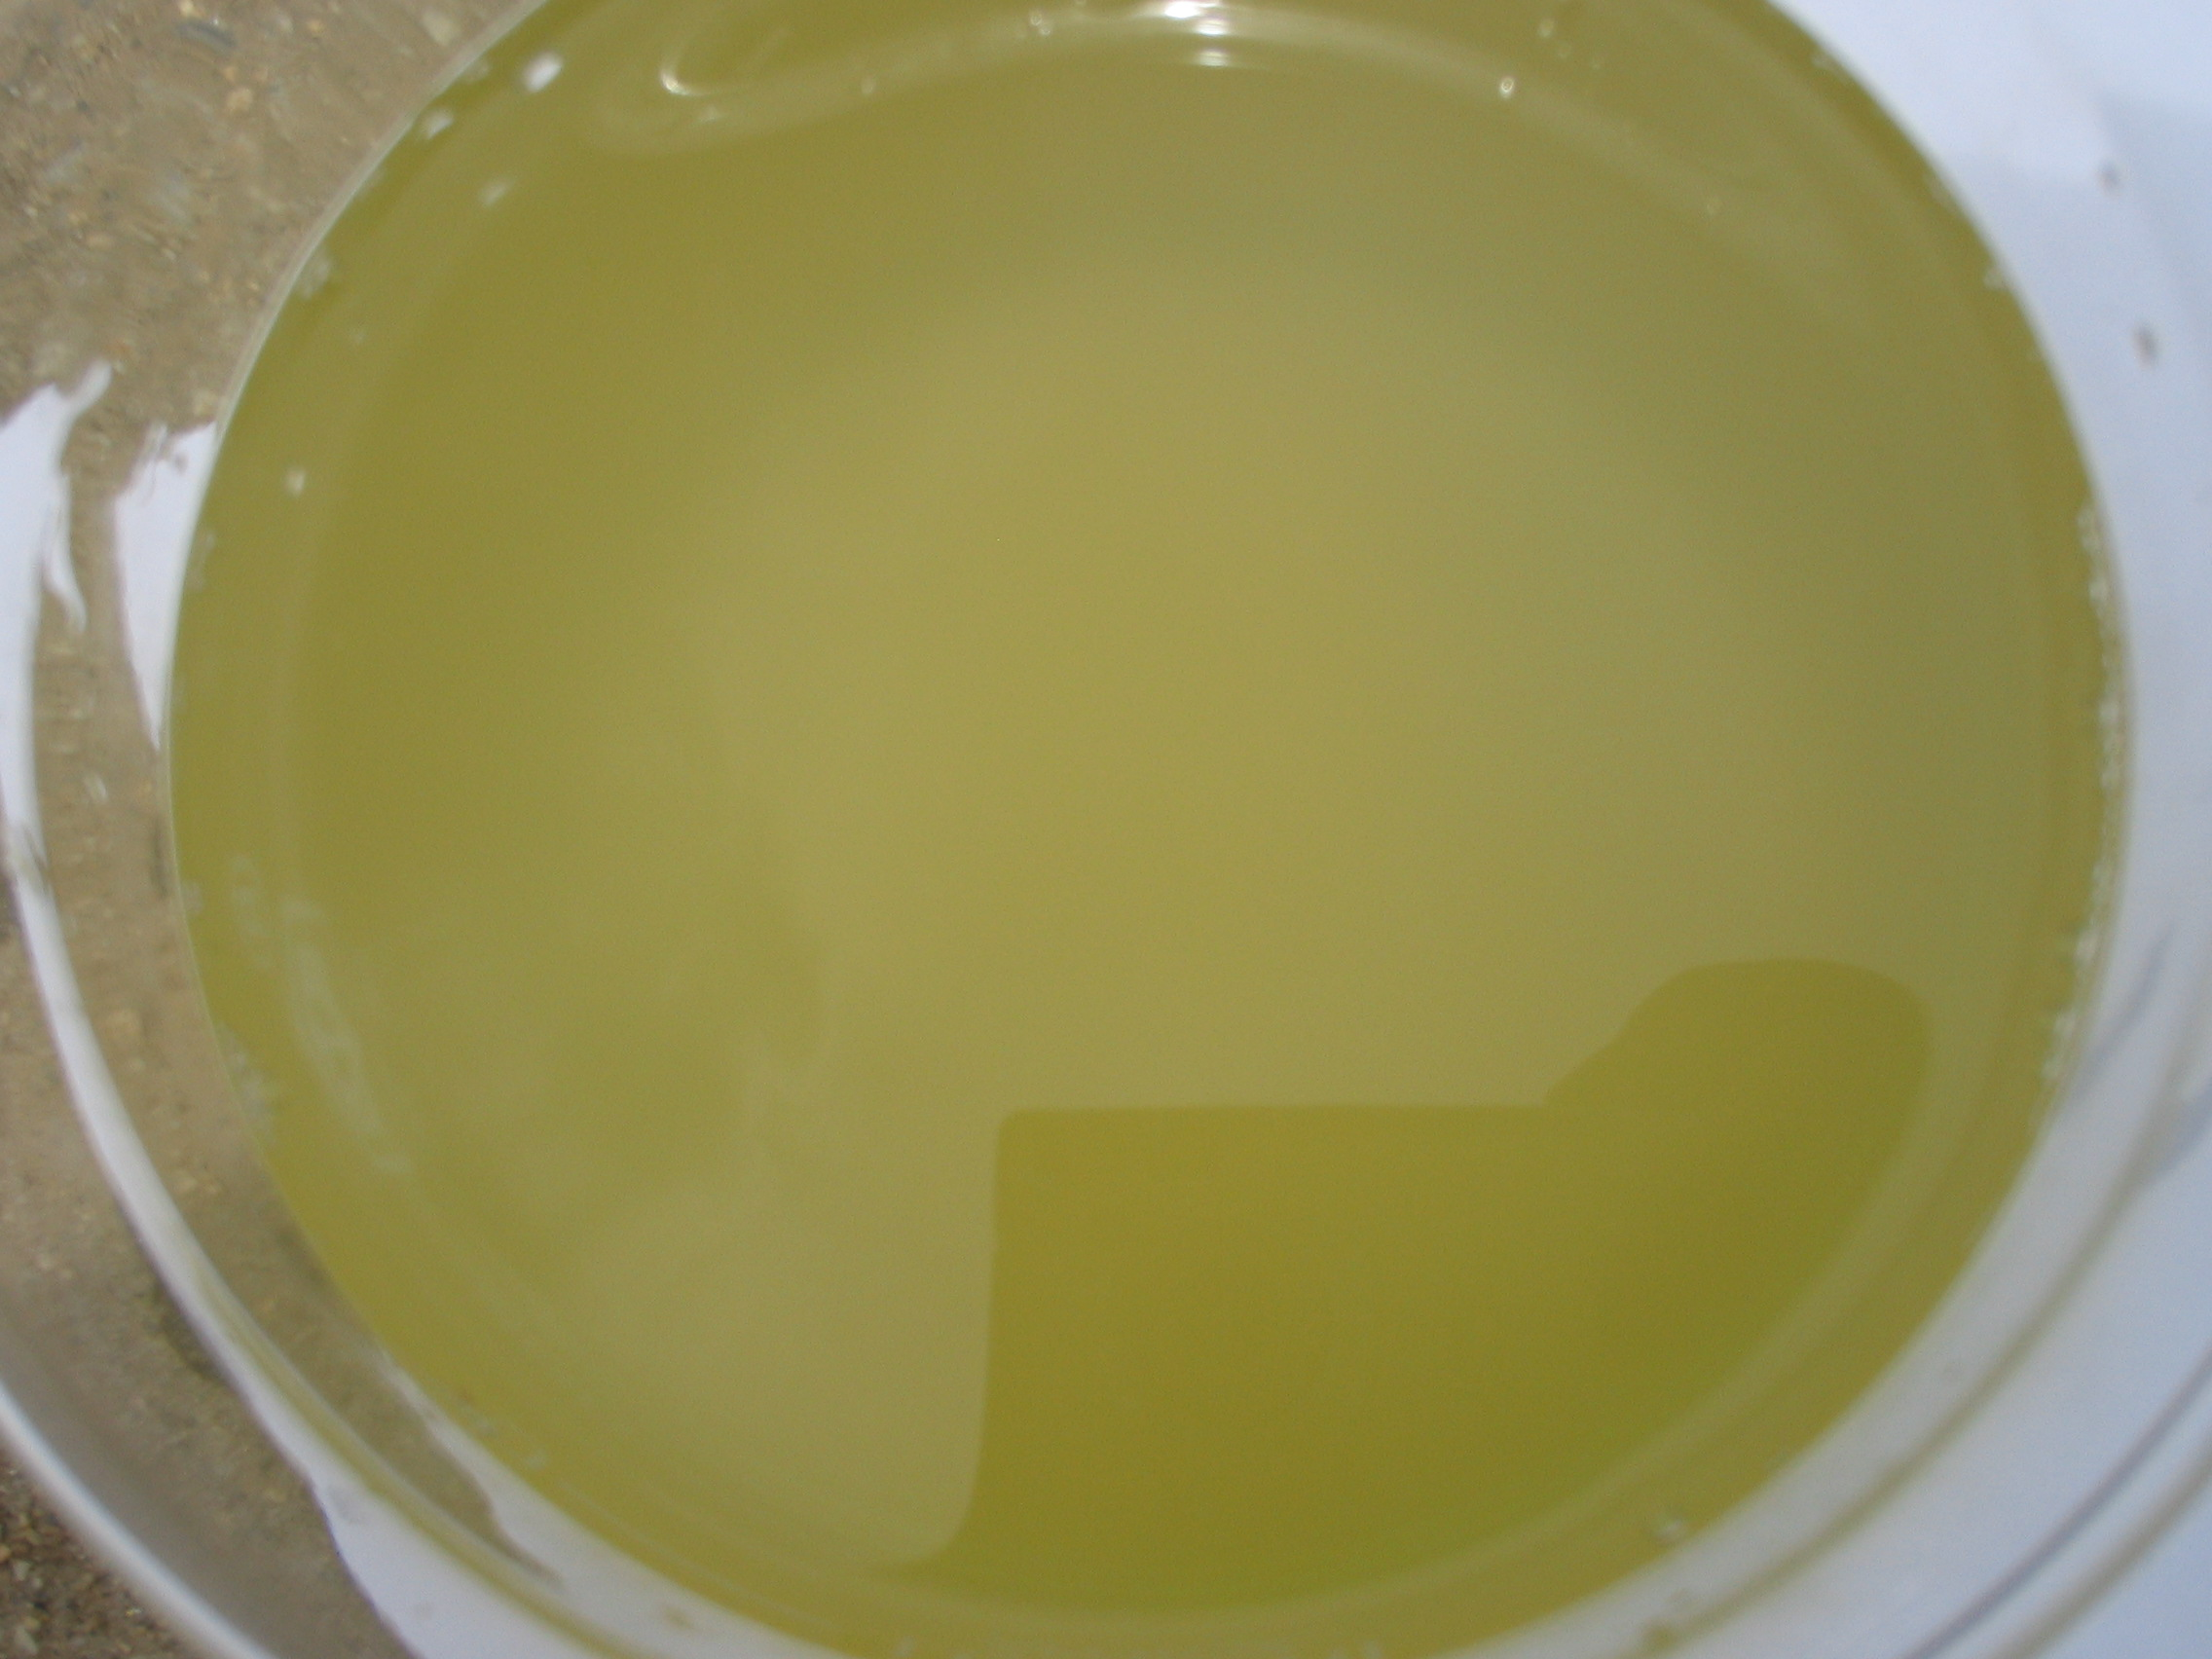
\includegraphics[width=6.3cm]{1_3.jpg}
		\centerline{$\ \ \ \ \ \ \ \ \ \ $(b)}
	\end{minipage}
	
	\caption{数据集}
\end{figure}

\subsection{数据预处理}


\subsubsection{图片裁剪}
\par 为了提取有效信息,规范数据输入,只裁剪中间含有有水质样本的图像。保留中心$100\times 100$的图像。
\begin{figure}[H]
	\centering
	\centerline{
\includegraphics[width=0.3\textwidth]{1_4.jpg}}  
	\begin{center}
		\caption{裁剪后}
	\end{center}
\end{figure}
\subsubsection{计算颜色矩}
\par 获取裁剪的图像后,对其RGB三个通道分别计算一到三阶颜色矩。之后采用str.split提取图片的类别,并将其存入Dataframe


\subsection{基于SVM的水质图片分类模型}
\par 对于此类小样本,采用SVM模型对其进行训练。	

\par 首先将预处理好的数据分割为训练集与测试集。之后调用sklearn.svm进行模型训练。



\subsection{模型结果}
\par 采取混淆矩阵对训练结果进行模型评价。可以看到SVM模型对1,2,3类水质预测较好。4,5类为不平衡数据。

\begin{figure}[H]
	\centering
	\centerline{\includegraphics[width=0.9\textwidth]{22_1}}  
	\begin{center}
		\caption{测试集混淆矩阵}
	\end{center}
\end{figure}




\newpage

\section{航空公司客户价值分析}
\subsection{数据集介绍}
\par 该数据为某航空公司客户信息,包含会员档案信息和其乘坐航班记录等信息。
\begin{figure}[H]
	\centering
	\centerline{\includegraphics[width=0.9\textwidth]{22_2}}  
	\begin{center}
		\caption{数据信息}
	\end{center}
\end{figure}
\begin{figure}[H]
	\centering
	\centerline{\includegraphics[width=0.9\textwidth]{22_3}}  
	\begin{center}
		\caption{流程图}
	\end{center}
\end{figure}

\subsection{数据预处理}
\par 首先,以2014-03-31为结束时间,选取宽度为两年的时间段作为分析观测窗口,抽取观测窗口内有乘机记录的所有客户的详细数据形成历史数据。对于后续新增的客户详细信息,利用其数据中最大的某个时间点作为结束时间,采用上述同样的方法进行抽取,形成增量数据。根据末次飞行日期,从航空公司系统内抽取2012-04-01至2014-03-31内所有乘客的详细数据,总共62988条记录

\par 原始数据中存在票价为空值,票价为空值的数据可能是客户不存在乘机记录造成。票价最小值为0、折扣率最小值为0、总飞行公里数大于0的数据。其可能是客户乘坐0折机票或者积分兑换造成。


\par 原始数据中属性太多,根据LRFMC模型,选择与其相关的六个属性,删除不相关、弱相关或冗余的属性。




\subsection{基于K-means的客户聚类}

\par 采用K-Means聚类算法对客户数据进行分群,将其聚成五类

\subsection{模型结果}
\par 对聚类结果进行特征分析,其中客户群1在F、M属性最大,在R属性最小;客户群2在L属性上最大;客户群3在R属性上最大,在F、M属性最小;客户群4在L、C属性上最小;客户群5在C属性上最大。

\begin{figure}[H]
	\centering
	\begin{minipage}[t]{0.48\textwidth}
		\centering
		\includegraphics[width=6.3cm]{22_4}
		\centerline{$\ \ \ \ \ \ \ \ \ \ $(a)}
	\end{minipage}
	\begin{minipage}[t]{0.48\textwidth}
		\centering
		\includegraphics[width=6.3cm]{22_5}
		\centerline{$\ \ \ \ \ \ \ \ \ \ $(b)}
	\end{minipage}
	
	\caption{结果可视化}
\end{figure}

\newpage

\section{基于用户的协同过滤}
\subsection{数据集说明}
\par 该数据包括IMDB用户对不同电影的打分情况,分为用户表,电影表,用户看过的电影及打分情况表。其中,打分情况表共100000行。
\subsection{相关系数的计算}
实现基于用户的协同过滤算法第一个重要的步骤就是计算用户之间的相似度。而计算相似度,建立相关系数矩阵目前主要分为以下几种方法。
\subsubsection{皮尔森相关系数}
皮尔逊相关系数一般用于计算两个定距变量间联系的紧密程度,它的取值在 [-1,+1] 之间。用数学公式表示,皮尔森相关系数等于两个变量的协方差除于两个变量的标准差。计算公式如下所示:
\begin{align}
	s(X, Y)=\frac{\operatorname{Cov}(X, Y)}{\sigma_{X} \sigma_{Y}}
\end{align}

由于皮尔逊相关系数描述的是两组数据变化移动的趋势,所以在基于 用户的协同过滤系统中,经常使用。描述用户购买或评分变化的趋势,若趋势相近则皮尔逊系数趋近于1,也就是我们认为相似的用户。
\subsubsection{基于欧几里德距离的相似度余弦相似度}
\par 欧几里德距离计算相似度是所有相似度计算里面最简单、最易理解的方法。计算出来的欧几里德距离是一个大于0的数,为了使其更能体现用户之间的相似度,可以把它规约到(0,1]之间,最终得到如下计算公式
\begin{align}
	s(X, Y)=\frac{1}{1+\sum \sqrt{\left(X_{i}-Y_{i}\right)^{2}}}
\end{align}
\par 只要至少有一个共同评分项,就能用欧几里德距离计算相似度;如果没有共同评分项,那么欧几里德距离也就失去了作用。其实照常理理解,如果没有共同评分项,那么意味着这两个用户或物品根本不相似。

\subsubsection{余弦相似度}
\par 余弦相似度用向量空间中两个向量夹角的余弦值作为衡量两个个体间差异的大小。余弦相似度更加注重两个向量在方向上的差异,而非距离或长度上。计算公式如下所示:
\begin{align}
s(X, Y)=\cos \theta=\frac{\vec{x} * \vec{y}}{\|x\| *\|y\|}
\end{align}

\subsection{基于用户的协同过滤}
\par 基于用户的协同过滤算法,另一个重要的步骤就是计算用户u对未评分商品的预测分值。首先根据上一步中的相似度计算,寻找用户u的邻居集N∈U,其中N表示邻居集,U表示用户集。然后,结合用户评分数据集,预测用户u对项i的评分,计算公式如下所示:
\begin{align}
p_{u, i}=\bar{r}+\frac{\sum_{u^{\prime} \subset N} s\left(u-u^{\prime}\right)\left(r_{u^{\prime}, i}-\bar{r}_{u^{\prime}}\right)}{\sqrt{\sum_{u^{\prime} \subset N}\left|s\left(u-u^{\prime}\right)\right|}}
\end{align}

其中,s(u- u')表示用户u和用户u'的相似度。
\subsection{算法的实现}
\par 现有的部分电影评分数据如下表 :
\begin{figure}[H]
	\centering
	\centerline{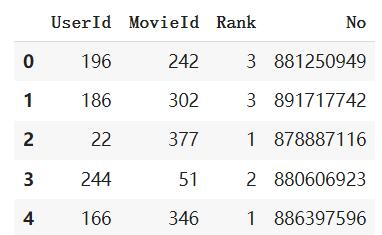
\includegraphics[width=0.5\textwidth]{72_1}}  
	\begin{center}
		\caption{部分数据}
	\end{center}
\end{figure}
\par 实现代码如下所示:
\begin{lstlisting}
def similarity(userid1:int,userid2:int,data:pd.DataFrame):
	# 获取userid1的电影id 并将其作为索引
	movie_index = list(data['MovieId'][data['UserId']==userid1].value_counts().index)
	
	#创建dataframe
	join_dataframe = pd.DataFrame(index=movie_index)
	
	#获取数据
	data1 = data[['MovieId','Rank']][data['UserId']==userid1].set_index('MovieId')
	data2 = data[['MovieId','Rank']][data['UserId']==userid2].set_index('MovieId')
	
	#换列名
	data1.columns = ['userid1']
	data2.columns = ['userid2']
	
	#join 连接
	join_dataframe = join_dataframe.join(data1)
	join_dataframe = join_dataframe.join(data2)
	join_dataframe = join_dataframe.fillna(0)
	
	# 计算相关系数
	norm1=np.sqrt(np.dot(join_dataframe['userid1'],join_dataframe['userid1']))
	norm2=np.sqrt(np.dot(join_dataframe['userid2'],join_dataframe['userid2']))
	val=np.dot(join_dataframe['userid1'],join_dataframe['userid2'])/(norm1*norm2)
	
	return val
	
c_user = 93
s = {}
all_user_id  = data['UserId'].unique()

for cid in all_user_id:
s[cid] = similarity(cid,c_user,data)
s[c_user] = 0
Max = max(s.items(),key=lambda x:x[1] if x[1]<=1 else 0)  # items以列表返回可遍历的(键, 值) 元组数组

Max = max(s.items(),key=lambda x:x[1] if x[1]<=1 else 0)  # items以列表返回可遍历的(键, 值) 元组数组

\end{lstlisting}

\subsection{模型结果}
\begin{figure}[H]
	\centering
	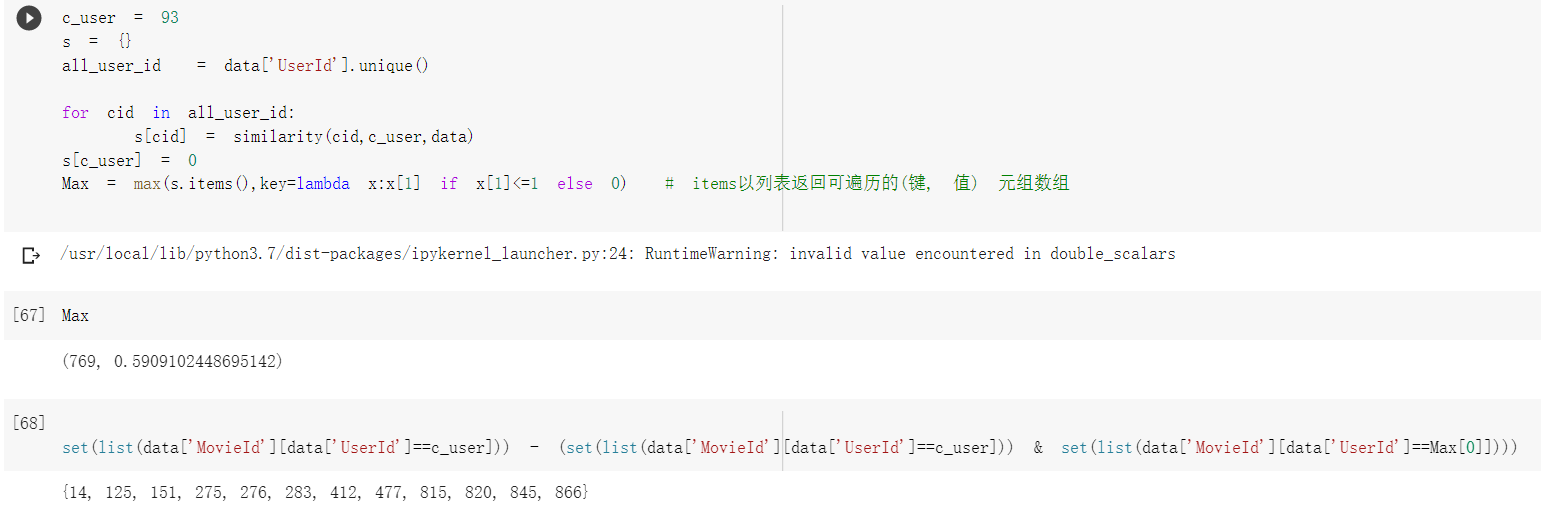
\includegraphics[width=0.7\linewidth]{figures/72_2}
	\caption{}
	\label{fig:722}
\end{figure}
\par 可以看到,与用户20最相似的为769,相似度为0.59,因此可以对20推荐{14, 125, 151, 275, 276, 283, 412, 477, 815, 820, 845, 866}电影。


\newpage
\section{中医证型的关联规则挖掘}

\subsection{数据集说明}
\par 该数据集为某机构收集的中医证型与乳腺癌阶段表,主要变量为六种证型(肝气郁结,热毒蕴结,冲任失调,气血两虚,脾胃虚弱,肝肾阴虚)与TNM分期。


\subsection{数据预处理}
\par 为了建模需要,需要对数据进行离散化。本例采用分箱对各个证型系数进行离散化处理,将每个属性聚成四类。
\par 
\par 实现代码如下所示:
\begin{lstlisting}
#数据预处理
columns = data.columns
key = list(columns)[0:6]
values = ['A','B','C','D','E','F']
dict(zip(key,values))
for i in range(6):
	cutbin = np.linspace(data[key[i]].min(),data[key[i]].max(),5)
	label = [values[i]+str(j) for j in range(1,5)]
	data[key[i]] = pd.cut(data[key[i]],bins=cutbin,labels=label)
\end{lstlisting}

\subsection{基于Apriori的关联规则挖掘}
\par 处理后的数据如下:

\begin{figure}[H]
	\centering
	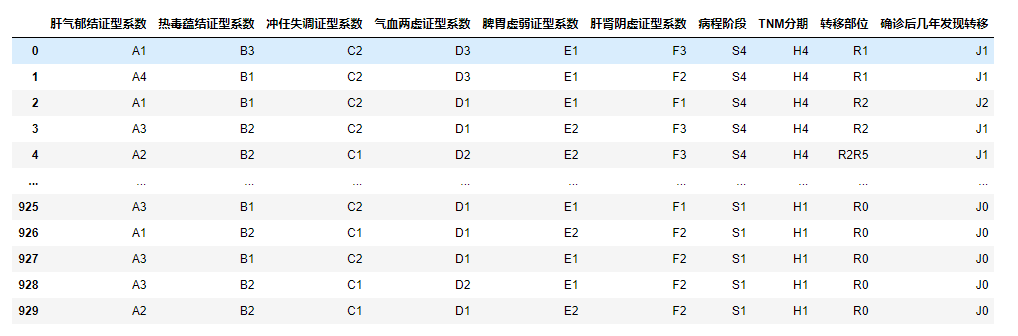
\includegraphics[width=\linewidth]{figures/731}
	\caption{}
	\label{fig:731}
\end{figure}

\par 

\subsection{模型结果与分析}
\par 设定最小支持度为0.07,最小置信度为0.9,结果为

{1: {('A1',): 111, ('S4',): 255, ('H4',): 415, ('J1',): 260, ('R2',): 80, ('J2',): 75, ('A3',): 275, ('A2',): 508, ('J3',): 80, ('S3',): 165, ('R0',): 515, ('J0',): 510, ('S2',): 340, ('S1',): 170, ('H3',): 205, ('H2',): 205, ('H1',): 105},\\
	
	 2: {('A1', 'J0'): 85, ('A1', 'R0'): 85, ('A2', 'H2'): 114, ('A2', 'H3'): 141, ('A2', 'H4'): 229, ('A2', 'J0'): 284, ('A2', 'J1'): 129, ('A2', 'R0'): 284, ('A2', 'S2'): 188, ('A2', 'S3'): 118, ('A2', 'S4'): 137, ('A3', 'H4'): 143, ('A3', 'J0'): 122, ('A3', 'J1'): 100, ('A3', 'R0'): 127, ('A3', 'S1'): 72, ('A3', 'S2'): 96, ('A3', 'S4'): 71, ('H1', 'J0'): 105, ('H1', 'R0'): 105, ('H2', 'J0'): 200, ('H2', 'R0'): 205, ('H2', 'S4'): 75, ('H3', 'J0'): 200, ('H3', 'R0'): 200, ('H3', 'S4'): 70, ('H4', 'J1'): 255, ('H4', 'J2'): 75, ('H4', 'J3'): 80, ('H4', 'R2'): 80, ('H4', 'S2'): 205, ('H4', 'S3'): 100, ('H4', 'S4'): 80, ('J0', 'R0'): 510, ('J0', 'S1'): 135, ('J0', 'S2'): 130, ('J0', 'S3'): 70, ('J0', 'S4'): 175, ('J1', 'S2'): 105, ('J1', 'S3'): 80, ('R0', 'S1'): 140, ('R0', 'S2'): 130, ('R0', 'S3'): 70, ('R0', 'S4'): 175}, \\
	 W
	3: {('A1', 'J0', 'R0'): 85, ('A2', 'H2', 'J0'): 114, ('A2', 'H2', 'R0'): 114, ('A2', 'H3', 'J0'): 141, ('A2', 'H3', 'R0'): 141, ('A2', 'H4', 'J1'): 129, ('A2', 'H4', 'S2'): 118, ('A2', 'J0', 'R0'): 284, ('A2', 'J0', 'S2'): 70, ('A2', 'J0', 'S4'): 103, ('A2', 'R0', 'S2'): 70, ('A2', 'R0', 'S4'): 103, ('A3', 'H4', 'J1'): 95, ('A3', 'J0', 'R0'): 122, ('H1', 'J0', 'R0'): 105, ('H2', 'J0', 'R0'): 200, ('H2', 'J0', 'S4'): 75, ('H2', 'R0', 'S4'): 75, ('H3', 'J0', 'R0'): 200, ('H3', 'J0', 'S4'): 70, ('H3', 'R0', 'S4'): 70, ('H4', 'J1', 'S2'): 100, ('H4', 'J1', 'S3'): 80, ('J0', 'R0', 'S1'): 135, ('J0', 'R0', 'S2'): 130, ('J0', 'R0', 'S3'): 70, ('J0', 'R0', 'S4'): 175}, \\
	
	4: {('A2', 'H2', 'J0', 'R0'): 114, ('A2', 'H3', 'J0', 'R0'): 141, ('A2', 'J0', 'R0', 'S2'): 70, ('A2', 'J0', 'R0', 'S4'): 103, ('H2', 'J0', 'R0', 'S4'): 75, ('H3', 'J0', 'R0', 'S4'): 70}}






\end{document} 